\documentclass[aspectratio=169]{beamer}


\usepackage[utf8]{inputenc}
\usepackage{amsmath}
\usepackage{amsfonts}
\usepackage{amssymb}
\usepackage{graphicx}
\usepackage{ragged2e}  % `\justifying` text
\usepackage{booktabs}  % Tables
\usepackage{tabularx}
\usepackage{tikz}      % Diagrams
\usetikzlibrary{calc, shapes, backgrounds}
\usepackage{amsmath}
\usepackage{amssymb}
\usepackage{dsfont}
\usepackage{url}       % `\url
\usepackage{listings}  % Code listings
\usepackage[T1]{fontenc}
\usepackage{nicematrix}
\usepackage{adjustbox}
\usepackage[utf8]{inputenc}
\usepackage[T1]{fontenc}
\usepackage{parskip}
\usepackage{graphicx}
\usepackage{media9}

\usepackage{graphicx}
\usepackage{sidecap}

\newcommand\setrow[1]{\gdef\rowmac{#1}#1\ignorespaces}

\usepackage{multicol}
\usepackage{theme/beamerthemehbrs}

\author{% 
Priya Chaudhary \\
Ragini Mishra \\ 
Sathwik Panchangam 
}
\title{General Solution To Find Objects}
\subtitle{D4, D5, D6 Final Demonstration}
\institute[HBRS]{Hochschule Bonn-Rhein-Sieg}
\date{\today}
\subject{Test beamer}
\def\advisors{Minh Nguyen \\
Alex Mitrevski
}


\begin{document}
{
\begin{frame}
\titlepage
\end{frame}
}

\begin{frame}{Contents}
\begin{enumerate}
  \item Project Goal
  \item Mid-term Deliverable
  \item Approach Used
  \item Project Changes
  \item Problems to be Solved
  \item Requirements
  \item Demo Video
  
\end{enumerate}
\end{frame}

\begin{frame}{Project Goal}
    \begin{multicols}{2}
        \begin{itemize}
            \item Find the user specified object.
            \item Use ontology to obtain the possible locations of the object.
            \item Navigate through possible locations.
            \item Perceive the scene and find the object.
            \item If object is not found move to next location and look for the object.
        \end{itemize}
        \vfill
        \begin{figure}[h!]
    	    \centering
    	    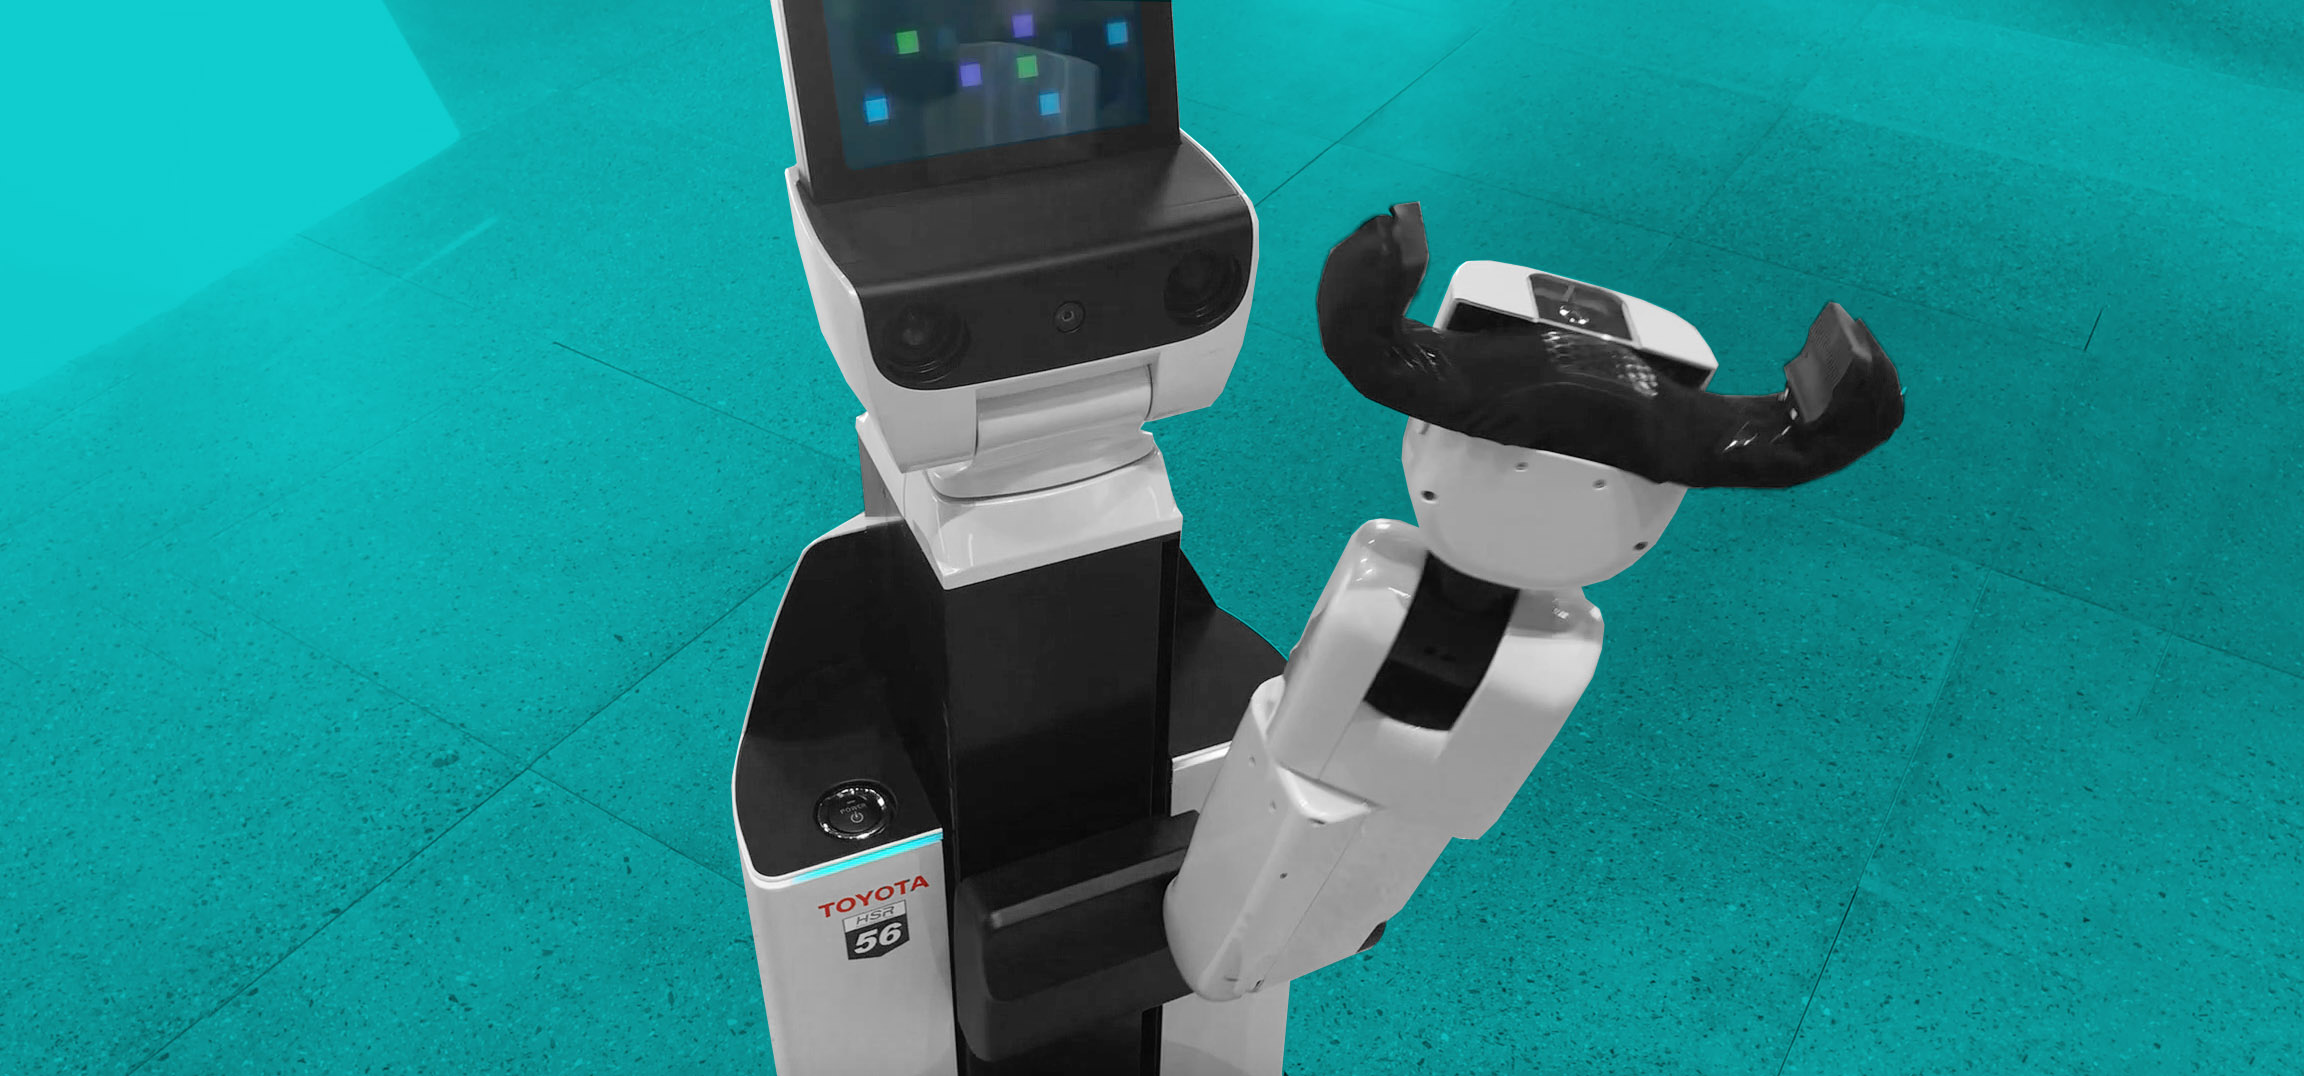
\includegraphics[width=40mm, scale=0.13]{hsr1.jpg}
    	    \caption{Toyota HSR robot}
        \end{figure}
        \begin{figure}
            \centering
            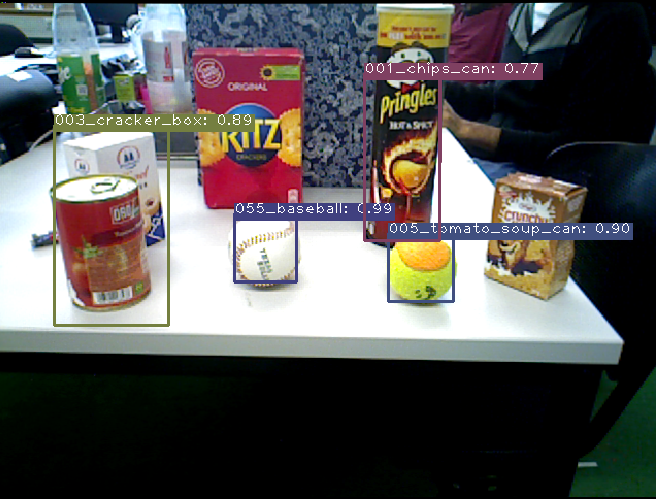
\includegraphics[width=40mm, scale =0.13]{final_demo_objects.png}
            \caption{Detected objects}
            \label{fig:my_label}
        \end{figure}
    \end{multicols}
\end{frame}

% \begin{frame}{The Project}
% \begin{itemize}
%     \item Given a user-specified choice(string), the software shall return all the default locations (strings) relative to the specified item based on the ontology structure.
%     \item Then interpret the default location in the ontology, and after obtaining the coordinates of the respective locations the robot shall navigate through all the respective returned locations(given the object is not found in the previous location).
%     \item Perceive the surfaces in all the locations to find the object and move on to the next location if the object is not found in the first location.
% \end{itemize} 
%   \begin{figure}[h!]
%     	\centering
%     	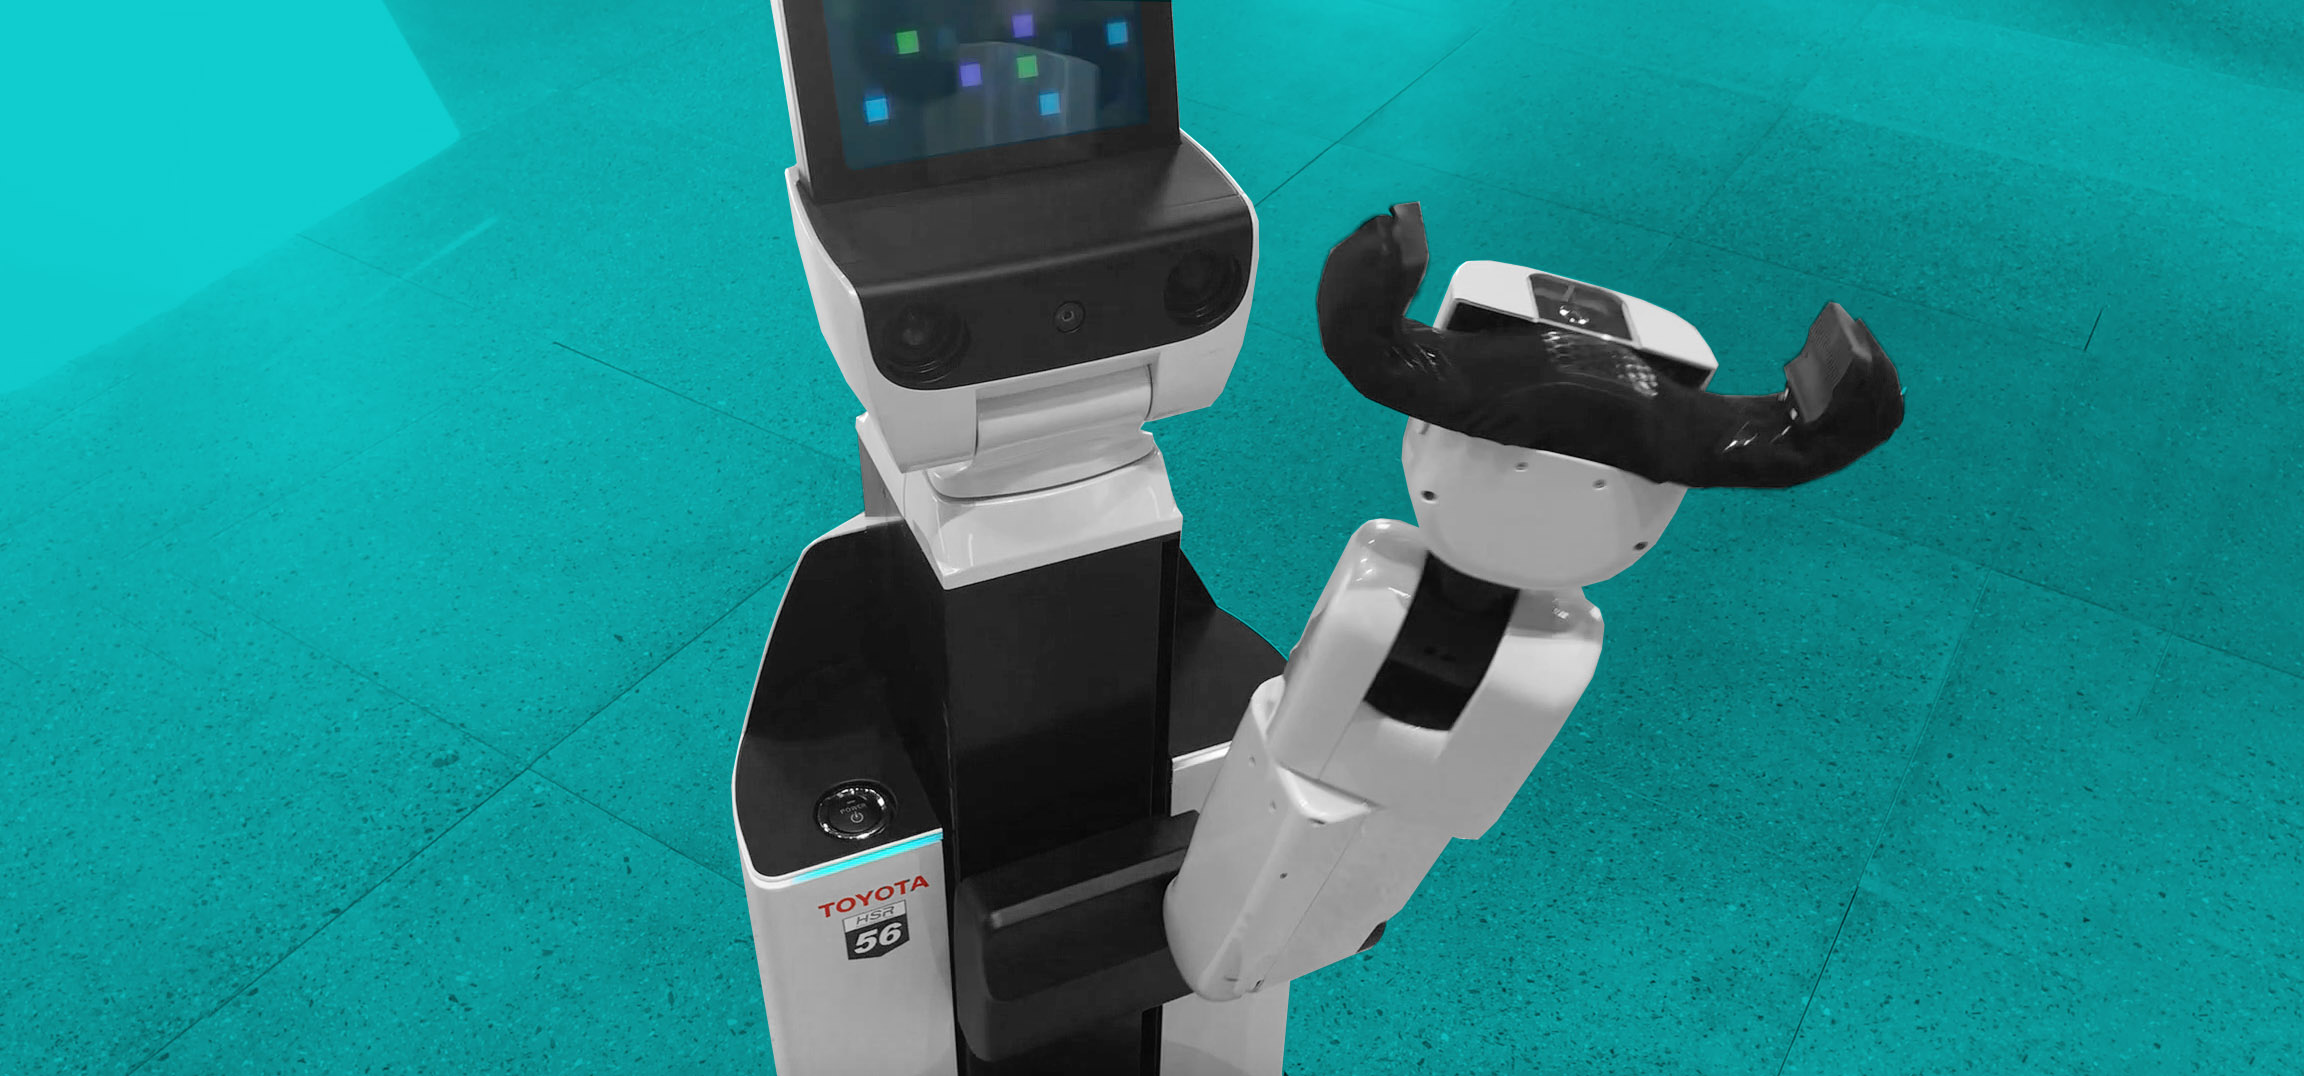
\includegraphics[width=50mm, scale=0.15]{hsr1.jpg}
% \end{figure}
% \end{frame}

\begin{frame}{Mid-term Deliverable}
      \begin{itemize}
        \item Updated ontology to return all the natural locations relative to the specified item.
        \item Mapped home lab and created natural locations and surfaces where the objects can found.
        \item Integrated navigation to find object package and the robot moves to all possible locations when an object name is given.
    \end{itemize}
    \vfill
\end{frame}

\begin{frame}{Approach Used}
    \begin{itemize}
    \item Implemented a general strategy to find a user-specified object
        \begin{itemize}
            \item Obtain the Possible locations of the user-specified object based on ontology.
        \end{itemize}
        \begin{multicols}{2}
        \begin{figure}
            \centering
            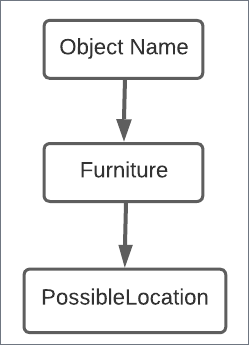
\includegraphics[width = 3cm, height= 3cm]{ontology.png}
            \caption{Basic structure}
            \label{fig:my_label}
        \end{figure}
        \begin{figure}
            \centering
            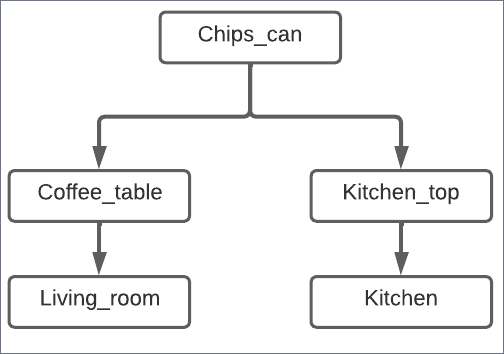
\includegraphics[width=3cm, height = 3cm]{ontology_final.png}
            \caption{Example}
            \label{fig:my_label}
        \end{figure}
        \end{multicols}
        \begin{itemize}
            \item Calculate the nearest possible location using the current location of the robot after localizing.
        \end{itemize}
    \end{itemize} 
    \vfill
\end{frame}
\begin{frame}{}
    \begin{itemize}
        \item Navigate through Possible Locations obtained from the ontology.
        \item Perceive the Furniture in the destination location using the perceive plane action and find the user specified object.
        \item If the object is found then pick up the object based on the perception results and pickup action.
        \item Move to next Possible Location and perceive the scene if the object is not found in the present location.
    \end{itemize}
\end{frame}

\begin{frame}{Project Changes}
 \framesubtitle{The changes made since mid-term:-}%
\begin{itemize}
    \item Added ycb objects to the ontology structure.
    \item Calculate the nearest possible location from the current location of the robot.
    \item Integrated perception to find object action package.
    \item Integrated pickup action to find object action package.
\end{itemize}
\end{frame}

\begin{frame}{Problems}
  \begin{itemize}
      \item Services need to be restarted for running the code for the second run.
      \begin{itemize}
          \item hsr\_move\_base\_action
          \item hsr\_move\_arm\_action
          \item hsr\_pickup\_action
      \end{itemize}
      \item Need to do a 2D pose estimate in rviz every time you run the code to get the current location coordinates.
      \item If the robot is not localized properly, the robot gets stuck near some obstacles.
  \end{itemize}
\end{frame}

\begin{frame}{}
    \begin{itemize}
      \item Rosplan\_interface stops working if the robot is force stopped before killing the running code.
      \item Need to delete the files in mongoDB\_store folder in mas\_knowledge\_base/common.
    \end{itemize}
    \begin{figure}
        \centering
        \includegraphics[width = 8cm,height=5cm]{mongo_error.png}
        \caption{MongoDB error - rosplan\_interface}
        \label{fig:my_label}
    \end{figure}
\end{frame}

\begin{frame}{}
    \begin{itemize}
        \item Misclassification of objects.
    \end{itemize}
    \begin{multicols}{3}
        \begin{figure}
            \centering
            \includegraphics[width =4cm,height=4cm]{misclassification1.png}
            \caption{misclassified objects}
            \label{fig:my_label}
        \end{figure}
        \begin{figure}
            \centering
            \includegraphics[width =4cm,height=4cm]{misclassification2.png}
            \caption{misclassified objects}
            \label{fig:my_label}
        \end{figure}
        \begin{figure}
            \centering
            \includegraphics[width =4cm,height=4cm]{missclassification3.png}
            \caption{misclassified objects}
            \label{fig:my_label}
        \end{figure}
    \end{multicols}
\end{frame}

\begin{frame}{Requirements}
    \begin{itemize}
        \item Ontology
        \item Navigation goals from the map as a YAML file
        \item Detector
        \item Dependent Packages
              \begin{itemize}
          \item hsr\_move\_base\_action
          \item hsr\_move\_arm\_action
          \item hsr\_pickup\_action
      \end{itemize}
    \end{itemize}
\end{frame}

\begin{frame}{Project Demo}
    \textbf{\begin{figure}[h!]
    	\centering
    	\includegraphics[width=4cm, height=6cm]{WhatsApp Image 2022-09-10 at 7.04.19 PM.jpeg}
%	\caption{Example structure }
\end{figure}}
\end{frame}

\begin{frame}{}
  \centering \Huge
  \emph{Thank You!}
\end{frame}

\end{document}